\chapter{Results} In this chapter, I analyze the benchmark results and discuss
their implications for data scientists using incremental random forest
classifiers. In each trial, each incremental random forest classifier received
batches sequentially, retraining itself after every new batch. For each tested
workload, I first contrast the performances of the incremental growth and tree
replacement strategies, and then I analyze a range of hybrid strategies and
explore the ideal hybrid strategy based on concept drift.

% TODO ERF


\section{Workload A: Large batches, no concept drift}

The Homesite Quote Conversion dataset is a Kaggle dataset that provides over
fifty numerical and categorical metrics on each of 200,000 customers. The
classification goal is to determine whether a potential customer will purchase
home insurance given the provided metrics about their quoted price, previous
activity, coverage information, and more. \cite{Homesite}

To study how incremental random forests would perform on workloads with large
batch sizes and no concept drift, I randomly divided the Homesite dataset into
ten batches of 20,000 data points each, and ran tests using both deep and
shallow random forests. By contrasting the error rates over time, I provide insight
into how these forests adapt over time.

\begin{figure}
  \centering
  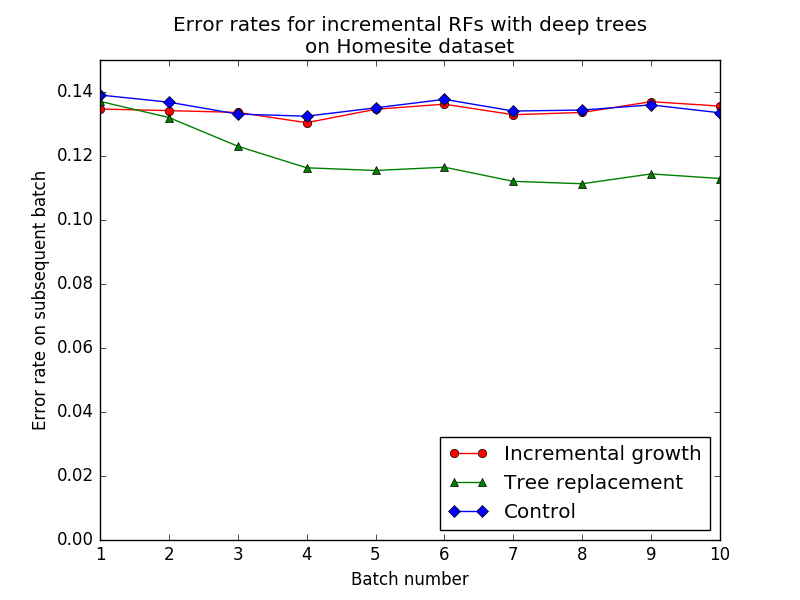
\includegraphics[width=4.0in]{g1}\\
  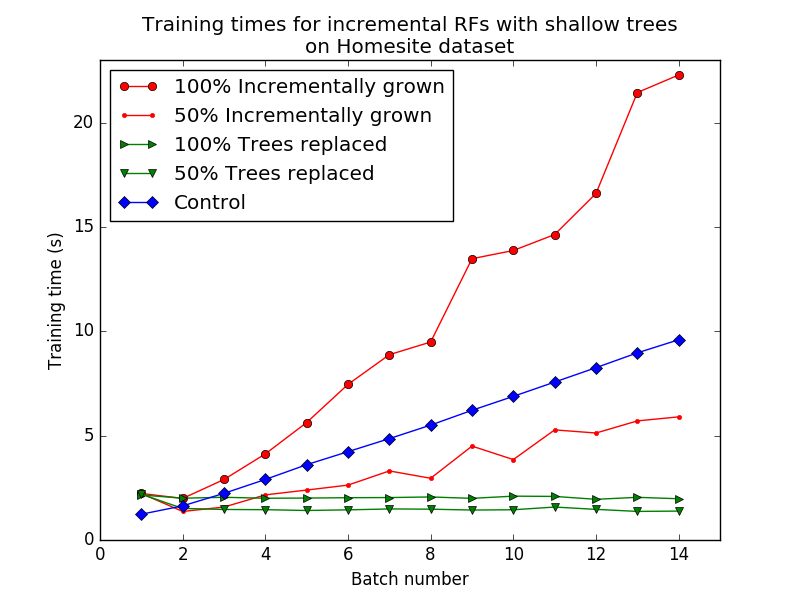
\includegraphics[width=4.0in]{g1_1}
  \caption{These graphs show the error rates and training times for the
  incremental growth strategy, the tree replacement strategy, and the control
  setting on the batched Homesite Quote Conversion dataset. In this benchmark,
  the random forest classifiers grow deep trees.}
  \label{fig:homesite}
\end{figure}

\begin{figure}
  \centering
  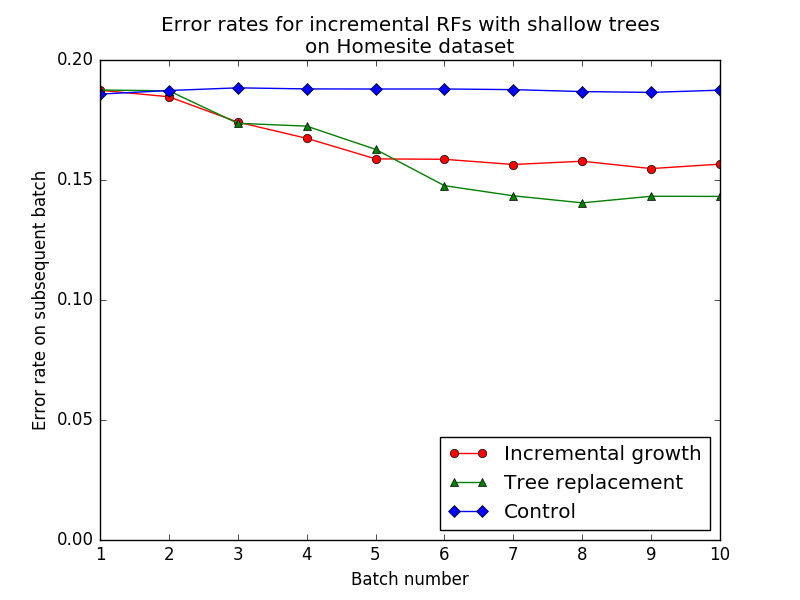
\includegraphics[width=4.0in]{g2}\\
  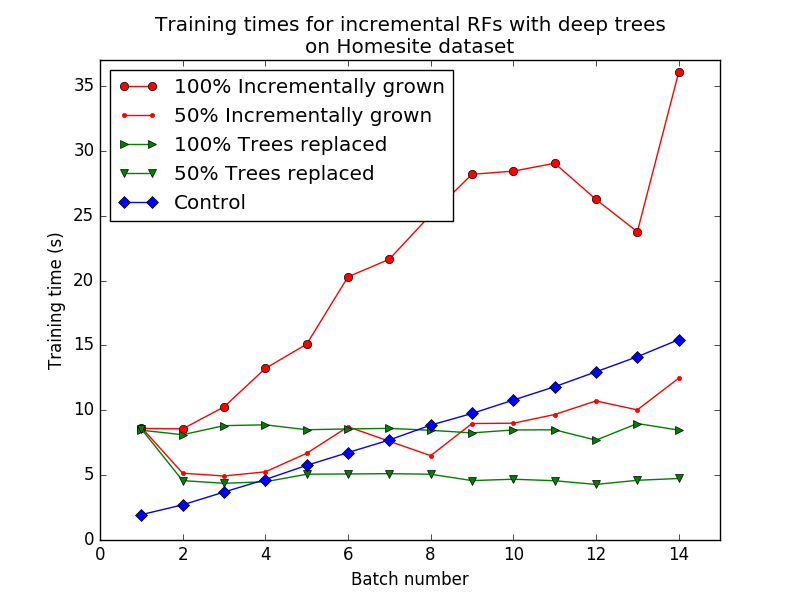
\includegraphics[width=4.0in]{g2_1}
  \caption{As with the graphs on the previous page, these graphs show the error
  rates and training times for the two experimental strategies, as well as the
  control. This benchmark, in contrast, measures random forest classifiers grown
  with shallow trees.}
  \label{fig:homesite2}
\end{figure}

As seen in Figures \ref{fig:homesite} and \ref{fig:homesite2}, in forests with
deep trees, the incremental growth strategy performed just as well as the
control, while the tree replacement strategy achieved an error rate over $2\%$
lower.  Because each batch contained 20,000 data points, the random forest
classifier was able to fit the data distribution accurately by just training on
the first batch of data. Since the dataset exhibited no concept drift, once the
data distribution was learned to a sufficient degree of accuracy, incrementally
growing each tree on new batches did not change the classification behavior of
the forest. As a result, the incremental growth strategy did not improve the
performance of the random forest. Similarly, incorporating each additional
batch into the tree by regrowing from scratch did not improve the accuracy of
the random forest.  However, the tree replacement strategy was able to better
fit to the data over time by replacing the trees with a lower overall
classification accuracy; since the batch size was large, if a tree had poor
classification performance on one batch, it likely would have poor performance
on future batches.

In contrast, in forests with shallow trees, the incremental growth strategy
performed far superior to the control, and almost as well as the tree
replacement strategy. Shallow trees more easily adapt to new data; in
traversing a decision tree from the root to a leaf, the information gain in
each leaf necessarily decreases with every level. Initially growing shallow
trees allows for future batches to more significantly impact the decisions made
by the forest.

As expected, retraining the entire tree from scratch on all data caused the
training time for the control setting to be much higher on later batches than
the training time for the experimental settings. The training times for the
incremental growth strategy were slightly smaller than the times for the tree
replacement strategy, regardless of tree depth.

Overall, for workloads such as the Homesite Quote Conversion batched dataset, a
large batch size and stationary distribution of data points indicates that a
pure replacement strategy is optimal to minimize error rate. 

TODO hybrid strategies

\begin{figure}
  \centering
  TODO
  \caption{These two plots show the average error rates of various hybrid tree
  replacement and incremental growth strategies on the Homesite batched
dataset. The axes indicate the percentage of trees that are modified according
to each strategy.}
  \label{fig:homesitehybrid}
\end{figure}

\section{Workload B: Small batches, no concept drift}

The Otto Group Product Classification dataset contains 200,000 data points
representing products sold by the Otto Group. Each data point is characterized
by nearly 100 numerical features representing qualities of each product; the
classification task is to distinguish one particular product category, ``Class
2,'' from the others. By randomly downsampling the dataset, I segmented the
data into batched workloads of approximately 100 points per batch, much smaller
than the 20,000-point batches of the Homesite dataset. \cite{Otto}

My initial analysis, as with the Homesite dataset, involved contrasting the
performance of the two incremental random forest strategies on the data. I
trained random forest classifiers using each of the two strategies on fifty
100-point batches of the Otto dataset to demonstrate any trends over time.

\begin{figure}
  \centering
  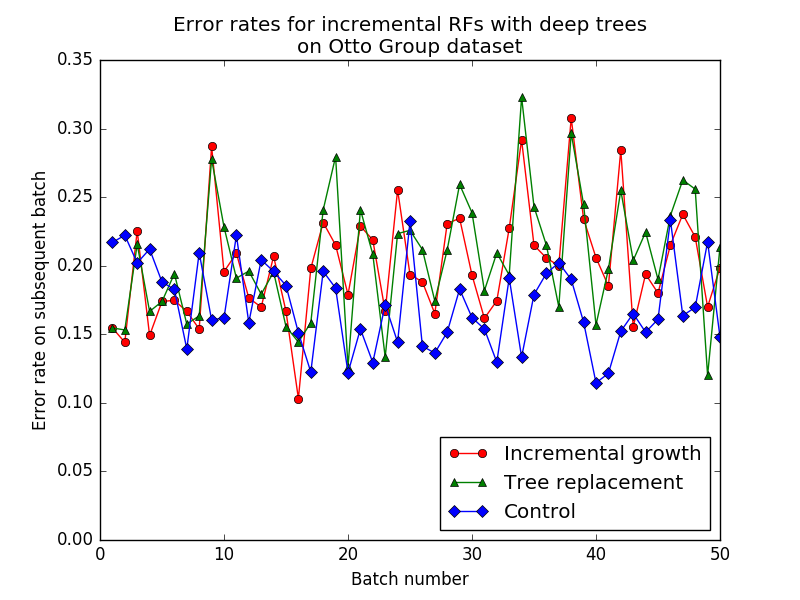
\includegraphics[width=4.0in]{otto3}\\
  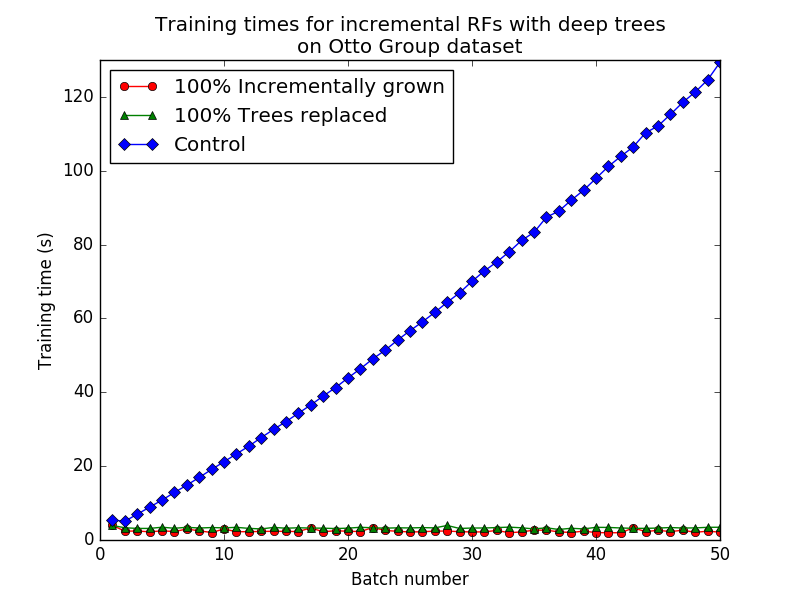
\includegraphics[width=4.0in]{otto4}
  \caption{These graphs show the error rates and training times for the
incremental growth strategy, the tree replacement strategy, and the control
setting on the batched Otto Group Product Classification dataset. These metrics
were taken on online random forest classifiers growing deep trees.}
  \label{fig:otto1}
\end{figure}

\begin{figure}
  \centering
  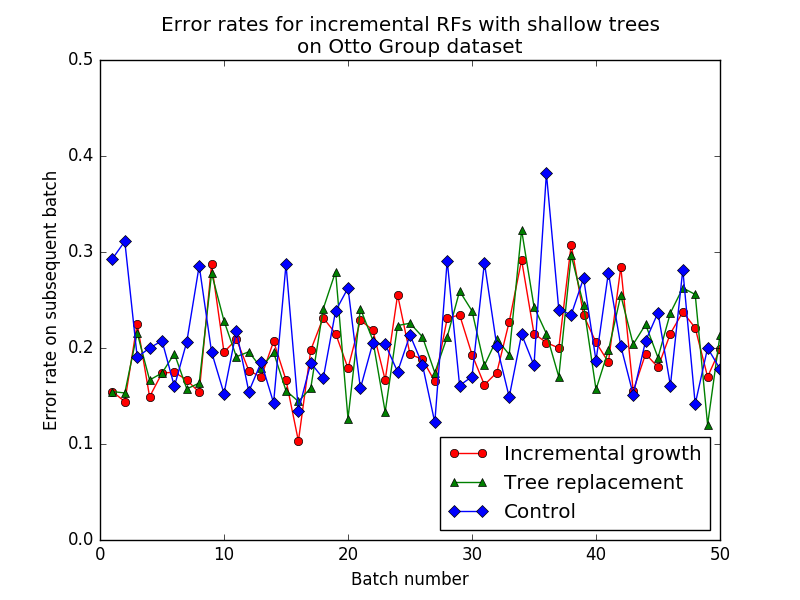
\includegraphics[width=4.0in]{otto1}\\
  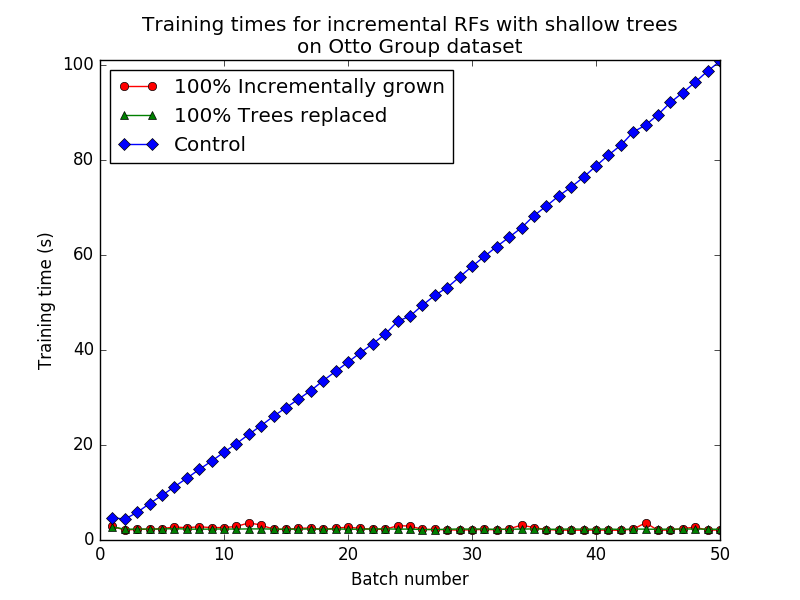
\includegraphics[width=4.0in]{otto2}
  \caption{As in the previous figure, these graphs show the error rates and
    training times for the two experimental strategies and the control on the
    Otto Group dataset. These benchmarks were measured on online random forest
  classifiers growing shallow trees.}
  \label{fig:otto2}
\end{figure}

As seen in Figures \ref{fig:otto1} and \ref{fig:otto2}, unlike with the Homesite
workload, there is no pure strategy that demonstrates the lowest error rate
across all batches. This observation is consistent both in random forest
classifiers with deep trees and in those with shallow trees. As expected, the
control again demonstrates the largest training time after each batch, as it
must be retrained from scratch on the aggregate data. 

\begin{figure}
  \centering
  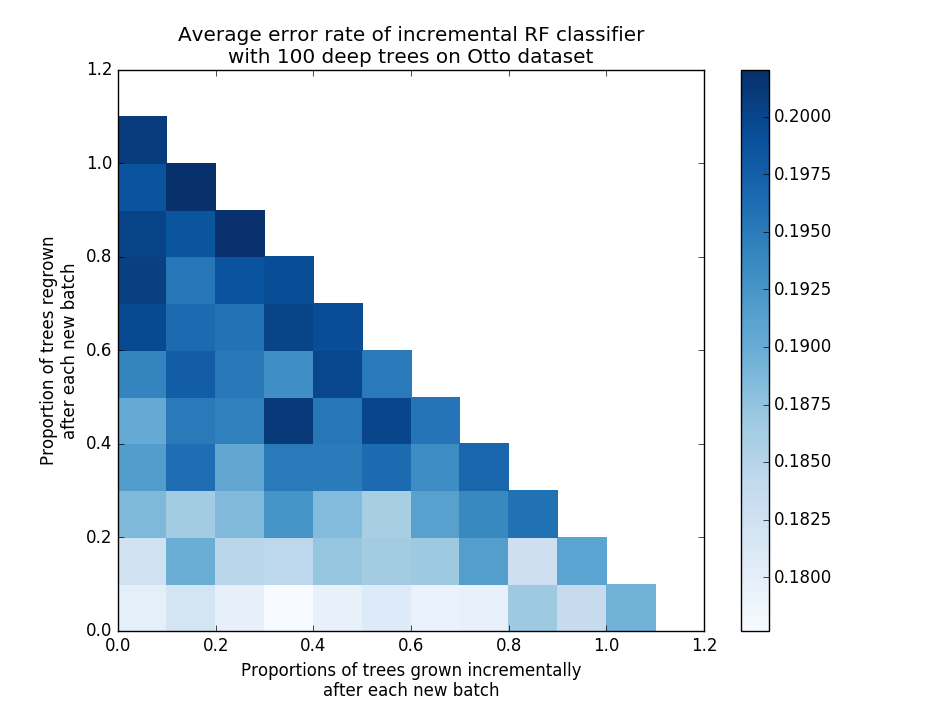
\includegraphics[width=5.0in]{otto_deep_med}\\
  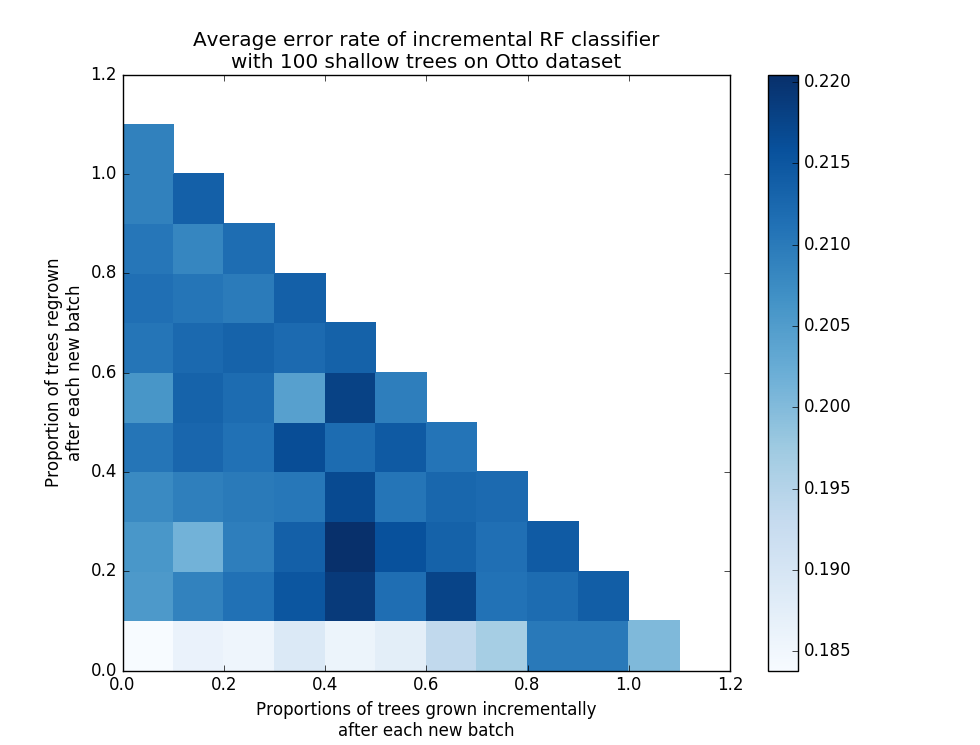
\includegraphics[width=5.0in]{otto_shallow_med}
  \caption{These two plots show the average error rates of various hybrid tree
  replacement and incremental growth strategies on the Otto Group batched
dataset. The axes indicate the percentage of trees that are modified according
to each strategy.}
  \label{fig:ottohybrid}
\end{figure}

Because the results do not indicate a clear dominant strategy, I instead
examine various hybrid approaches---strategies that combine both incrementally
growing and replacing trees.  As seen from the data in Figure
\ref{fig:ottohybrid}, for smaller batch sizes such as 100, strategies that
involve only incremental growth generally perform better than strategies that
incorporate some proportion of regrown trees. This trend is present in both
random forest classifiers comprised of deep trees and those with shallow trees,
though the trend is stronger among forests with shallow trees. 

Trees grown on one batch naturally overfit to that batch. With a small batch
size, there is a higher likelihood that data distribution differs from the
overall data distribution of the full dataset. As such, tree replacement
strategies could grow trees that fit well to one batch, but that fit poorly to
the rest of the data, increasing the error rate. Incremental growth
incorporates the data from multiple batches into each tree, mitigating the
effect of overfitting to the wrong data distribution.

Overall, these results demonstrate that data scientists using incremental
random forests on workloads with small data batches should utilize a strategy
that only involves incremental growth. Figure \ref{fig:ottohybrid} indicates
that the specific proportion of trees that are incrementally grown can vary
with little impact on accuracy, so data scientists should choose a smaller
ratio to minimize training time.

\section{Workload C: Large batches, concept drift}

The US Department of Transportation Airline On-Time Statistics and Delay Causes
dataset contains information about every flight that took place in the last
decade. I used 18-months of this dataset, beginning in January 2014, for my
analysis. Because the distribution of airline delay data varies seasonally,
this dataset exhibits concept drift. Each month of data translated to a
10,000-point batch in an 18-batch data workload. \cite{Plane}

\begin{figure}
  \centering
  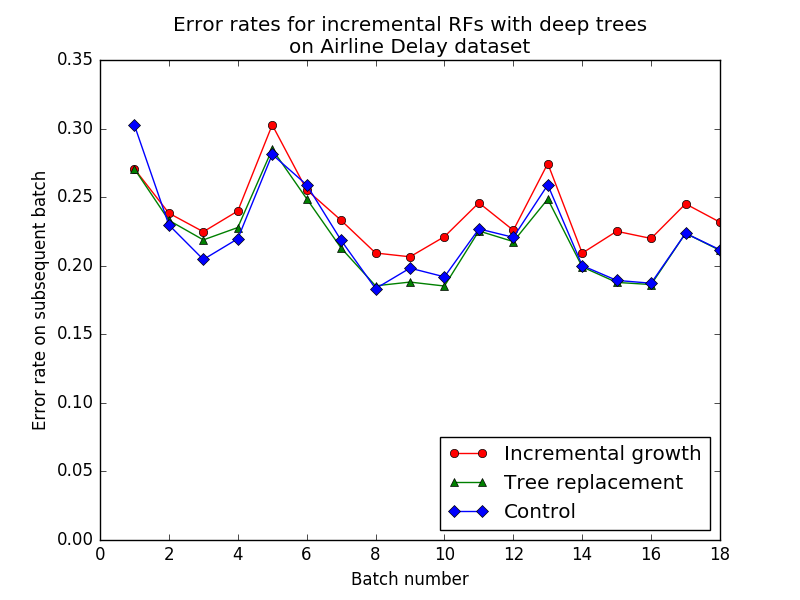
\includegraphics[width=4in]{planedeep_line}
  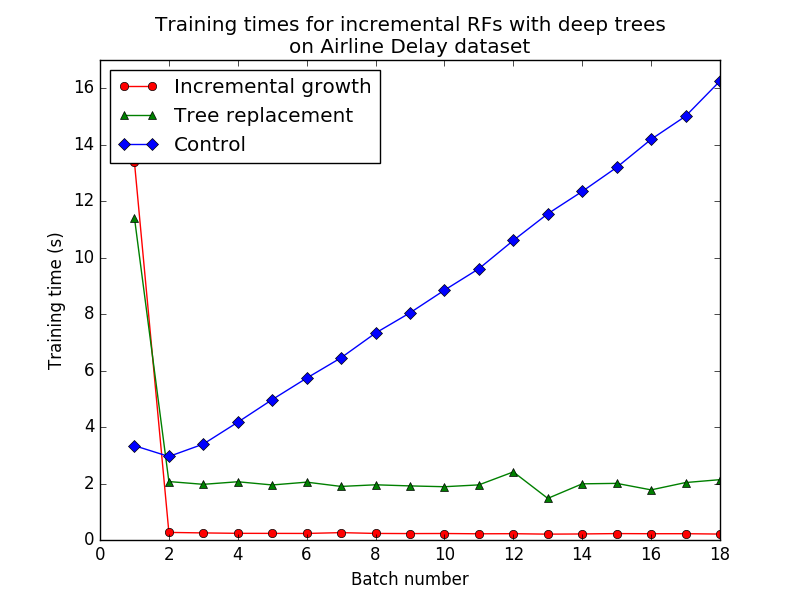
\includegraphics[width=4in]{planedeep_line_time}
  \caption{airline data}
  \caption{These graphs show the error rates and training times for the
incremental growth strategy, the tree replacement strategy, and the control
setting on the batched Airline Delay dataset. These metrics
were taken on online random forest classifiers growing deep trees.}
  \label{fig:plane1}
\end{figure}

\begin{figure}
  \centering
  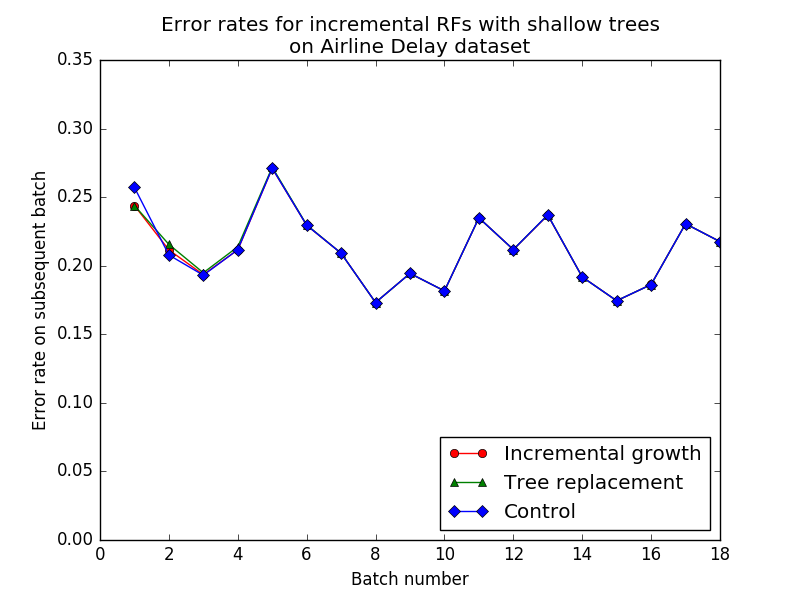
\includegraphics[width=4in]{planeshallow_line}
  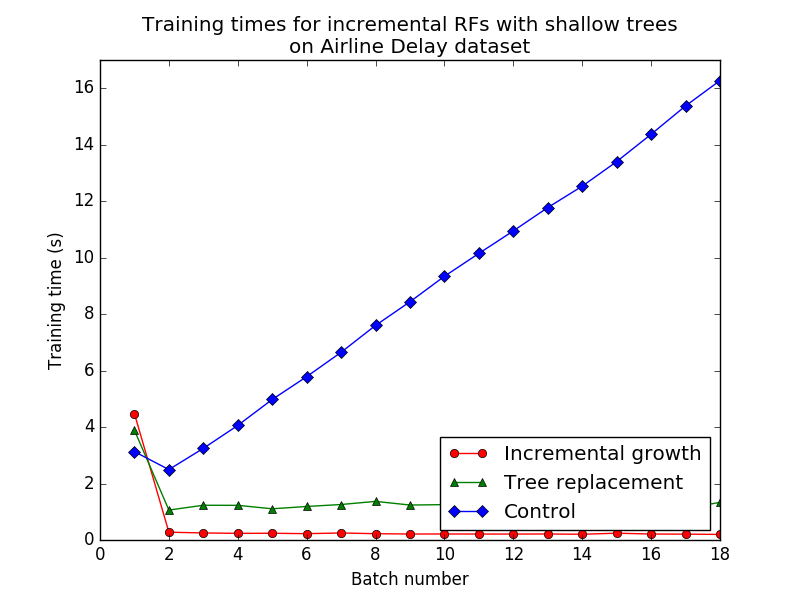
\includegraphics[width=4in]{planeshallow_line_time}
  \caption{airline data}
  \caption{As in the previous figure, these graphs show the error rates and
    training times for the two experimental strategies and the control on the
    batched Airline Delay dataset. These benchmarks were measured on online random forest
  classifiers growing shallow trees.}
  \label{fig:plane2}
\end{figure}


TODO plane data analysis


\begin{figure}
  \centering
  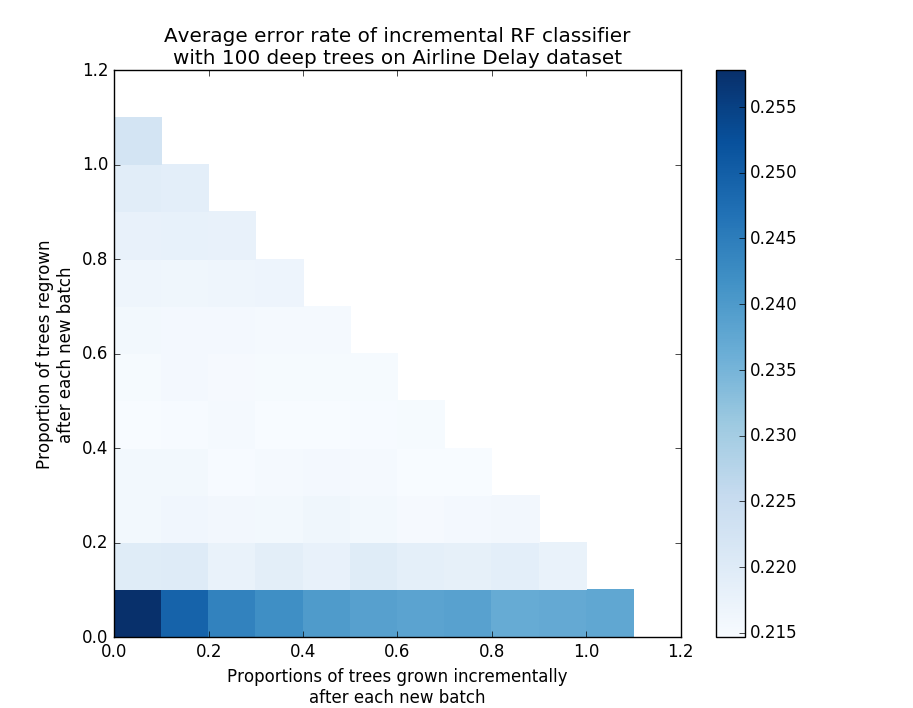
\includegraphics[width=5in]{planedeep}
  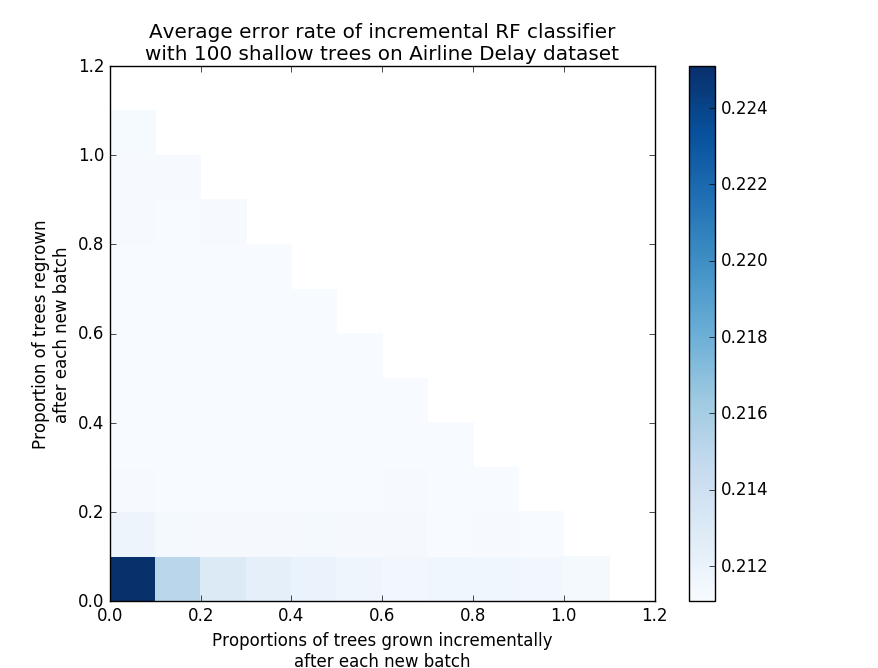
\includegraphics[width=5in]{planeshallow}
  \caption{These two plots show the average error rates of various hybrid tree
  replacement and incremental growth strategies on the Airline Delay batched
dataset. The axes indicate the percentage of trees that are modified according
to each strategy.}
  \label{fig:planehybrid}
\end{figure}
 
TODO force extreme concept drift with otto dataset



\section{Workload D: Small batches, concept drift}


TODO plane data analysis


\begin{figure}
  \centering
  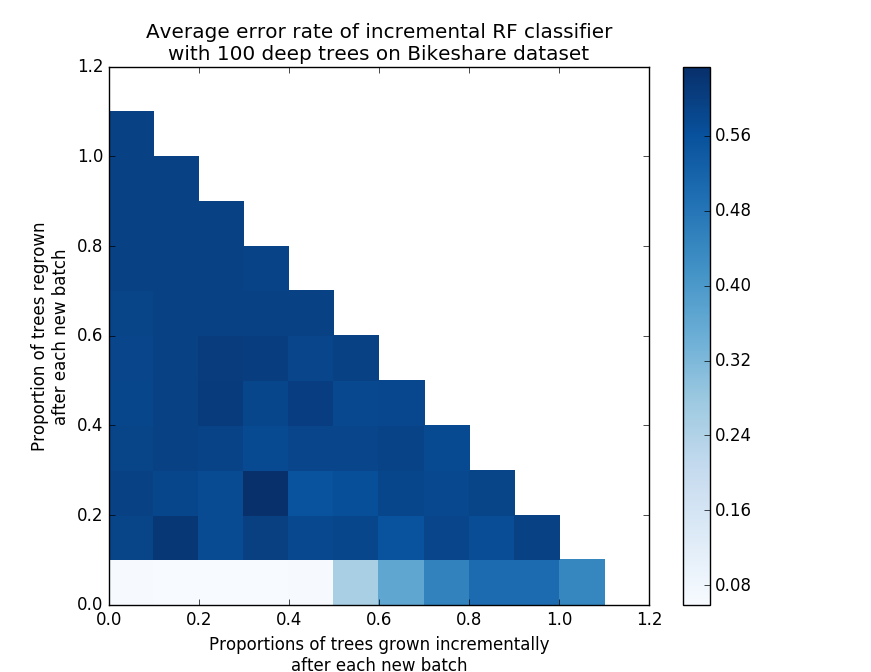
\includegraphics[width=5in]{bikesharedeep}
  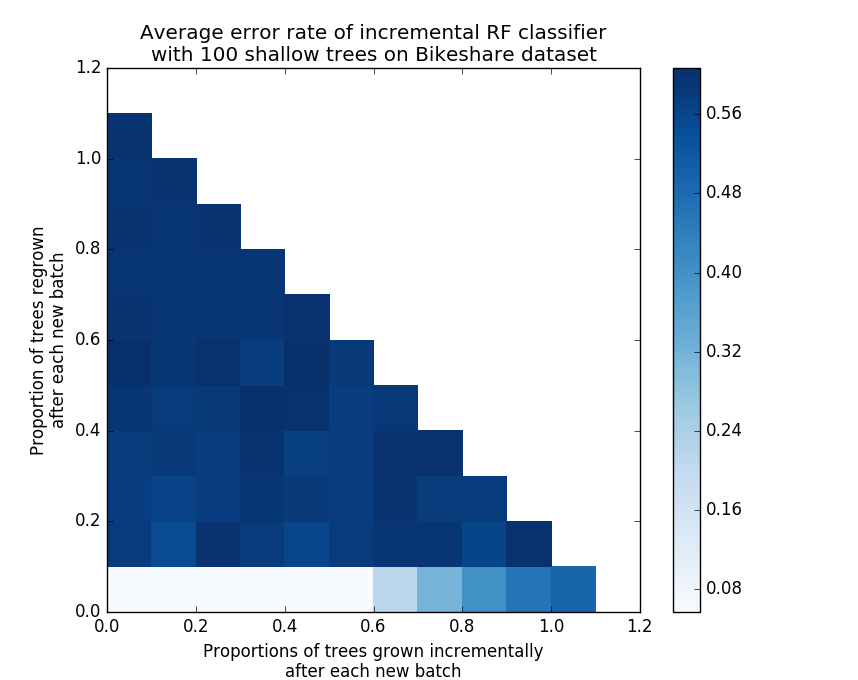
\includegraphics[width=5in]{bikeshareshallow}
  \caption{These two plots show the average error rates of various hybrid tree
  replacement and incremental growth strategies on the Bike Sharing batched
dataset. The axes indicate the percentage of trees that are modified according
to each strategy.}
  \label{fig:bikesharehybrid}
\end{figure}
 

